\documentclass{article}
\usepackage[utf8]{inputenc}
\usepackage[portuguese]{babel}
\usepackage[a4paper, total={6in, 8in}]{geometry}
\usepackage{graphicx}
\usepackage{float}
\usepackage[title]{appendix}
\usepackage[style=numeric]{biblatex}
\usepackage{csquotes}
\usepackage{mathtools}
\usepackage{xcolor}
\usepackage{minted}
\usepackage{framed}
\addbibresource{references.bib}

\begin{document}

{
\center
\begin{figure}[H]
        \centering
        
\includegraphics[width=3cm]{Pictures/UM_EENG.jpg}
\end{figure}
\textsc{\Large Universidade do Minho} \\ [0.5cm]
\textsc{\Large Mestrado em Engenharia Informática} \\ [0.5cm]
\textsc{\large Scripting no Processamento de Linguagem Natural} \\ [0.5cm]

{\LARGE \bfseries Polyglot - Framework NLP} \\[0.5cm]

\begin{tabular}{c c}
    Diana Ribeiro Barbosa & José Carlos Lima Martins \\
    A78679 & A78821 \\
\end{tabular} \\[0.5cm]

\today \\[1cm]
}

\tableofcontents

\newpage
\section{Introdução}
\qquad O presente trabalho foi desenvolvido no âmbito da unidade curricular Scripting no Processamento de Linguagem Natural, do perfil de especialização Processamento de Linguagens e Conhecimento do 4º ano do Mestrado Integrado em Engenharia Informática da Universidade do Minho.
\par O objetivo do mesmo é a exploração de uma ferramenta para Processamento de Linguagem Natural, neste caso, uma framework em \textit{Python}, a linguagem de eleição da disciplina. A ferramenta em questão é o \textit{Polyglot}.
\par Assim, ao longo deste relatório, fazemos uma  introdução à \textit{framework}, às funcionalidades disponibilizadas pela mesma e aos seus componentes, organização e estrutura interna. Elaboramos ainda um pouco sobre aspetos mais práticos, como a sua instalação, exemplos da sua implementação e o suporte em português para a mesma, bem como damos sugestões de ideias relacionadas que não chegamos a implementar no projeto.


\section{O que é o \textit{Polyglot?}}

\quad O \textit{Polyglot} é uma biblioteca em \textit{Python} desenvolvida por Rami Al-Rfou em conjunto com Bryan Perozzi e Steven Skiena, cujo objetivo é facilitar tarefas de Processamento de Linguagem Natural. Apesar de não ser tão conhecida como, por exemplo, a NLTK (\textit{Natural Language Toolkit}) e a \textit{Spacy} \cite{comparacoes}, possui várias funcionalidades que podem ser utilizadas em aplicações multi-línguas, cobrindo para cada uma destas funcionalidades entre 16 a 137 idiomas únicos.


\section{Funcionalidades disponibilizadas}
As oito funcionalidades disponibilizadas pelo \textit{Polyglot} são as seguintes:

\paragraph{Tokenização:} Esta funcionalidade (disponível para 165 línguas) está dividida em duas partes principais: a segmentação do texto input em frases e a identificação das palavras que constituem cada uma. Estas podem ser feitas em qualquer ordem, isto é, primeiro a tokenização das palavras e posteriormente a segmentação em frases ou vice-versa\cite{tokenization}.

\paragraph{Deteção da língua:} O \textit{Polyglot} consegue identificar um total de 196 línguas diferentes dado um texto input. Caso haja mais de uma língua no mesmo texto, ou não haja informação suficiente para uma deteção o polyglot devolve ainda o nível de confiança associado às suas previsões\cite{langdetect}.

\paragraph{Reconhecimento/extração de entidades mencionadas:} Capacidade de reconhecer/extrair de um texto menções a locais (cidades, países, regiões, continentes, divisões administrativas,...), organizações (equipas desportivas, jornais de notícias, bancos, universidades, escolas, empresas,...) e personalidades relevantes (políticos, cientistas, artistas, atletas, empreendedores, ... ). Estas entidades foram extraídas de datasets da \textit{Wikipédia} em 40 línguas\cite{nae}.

\paragraph{Identificação de categorias gramaticais:} Atribuição a cada palavra de uma categoria que identifica a funcionalidade sintática da mesma no texto. Esta pode ser uma de 17 tipos: adjetivo, adposição, advérbio, verbo auxiliar, conjunção coordenativa, determinante, interjeição, substantivo, numeral, partícula, pronome, nome próprio, pontuação, conjunção subordinada, símbolo, verbo e outro (caso não se enquadre em nenhuma das anteriores). O \textit{Polyglot} suporta esta funcionalidade em 16 idiomas\cite{post}.

\paragraph{Análise de Sentimento:} O \textit{polyglot} oferece ainda uma funcionalidade particularmente interessante para o processamento de linguagem natural a nível da análise semântica de textos (estudo e interpretação do significado de uma palavra, frase ou de uma expressão num determinado contexto). Concretamente, através da atribuição de polaridades. A escala contém 3 graus: +1 para palavras positivas, -1 para palavras negativas e 0 para palavras neutras. Esta análise é possível para palavras de 136 idiomas e permite o cálculo de sentimento associado às entidades mencionadas\cite{sent}.

\paragraph{\textit{Embedding} de palavras:} Mapeamento de uma palavra para um espaço vetorial d-dimensional de valor real de modo a capturar recursos semânticos e sintáticos. Isto é, é uma representação de palavras que permite que termos com significados semelhantes sejam representados de forma semelhante. Assim, é possível por exemplo calcular vizinhos de palavras, ou seja, palavras cujo significado está relacionado (podem ser agrupadas numa categoria). Esta funcionalidade está disponível em 137 linguagens\cite{emb}.

\paragraph{Análise Morfológica:} A análise morfológica consiste na identificação de morfemas (por exemplo o prefixo, o radical e o sufixo) a partir das palavras. Os morfemas são as unidades mais pequenas das línguas e o \textit{Polyglot} treinou os seus modelos nas 50000 palavras mais frequentes de 135 idiomas. Esta funcionalidade é útil também na deteção de idiomas já que há muitas palavras com várias formas diferentes e extrair o radical desses casos através deste tipo de análise pode ajudar a identificar a língua através das palavras associadas a esta\cite{ma}.

\paragraph{Transliteração:} A transliteração consiste na reescrita de um texto escrito numa dada linguagem com um determinado alfabeto para outro alfabeto, sendo portanto diferente de uma tradução. O \textit{polyglot} cobre 69 linguagens diferentes abrangendo vários alfabetos. Isto é particularmente útil por exemplo para um utilizador com um dado teclado conseguir escrever numa linguagem cujo teclado não está preparado para o fazer (sendo possível devido por exemplo ao uso de acentos)\cite{translit}. 


\section{Componentes, Organização e Estrutura}
\qquad
De forma a suportar algumas das funcionalidades para uma dada língua, é necessário fazer download através da \textit{framework} dos ficheiros necessários, eg.:
\begin{verbatim}
    polyglot download transliteration2.pt
\end{verbatim}
O código acima realizaria o download dos ficheiros necessários para a funcionalidade de transliteração em texto escritos em língua portuguesa.

A framework é gratuita, possuindo uma licença GPLv3. Quanto à sua documentação, esta está presente em \url{http://polyglot.readthedocs.org}. Para além disso, o \textit{Polyglot} possui um repositório no GitHub disponível em  \url{https://github.com/aboSamoor/polyglot}.

Esta ferramenta possui duas formas de interagir com a mesma: através na biblioteca em Python ou através da linha de comandos. No anexo \ref{helpCMD} está presente o menu de ajuda da interface via linha de comandos.

Quanto à estrutura do Polyglot (Package) o mesmo está divido em sub-packages e em sub-módulos \cite{modulos}:
\begin{itemize}
    \item sub-packages
    \begin{itemize}
        \item Package polyglot.detect
        \begin{itemize}
            \item sub-módulos
            \begin{itemize}
                \item Módulo polyglot.detect.base
                \item Módulo polyglot.detect.langids
            \end{itemize}
        \end{itemize}
        \item Package polyglot.mapping
        \begin{itemize}
            \item sub-módulos
            \begin{itemize}
                \item Módulo polyglot.mapping.base
                \item Módulo polyglot.mapping.embeddings
                \item Módulo polyglot.mapping.expansion
            \end{itemize}
        \end{itemize}
        \item Package polyglot.tag
        \begin{itemize}
            \item sub-módulos
            \begin{itemize}
                \item Módulo polyglot.tag.base
            \end{itemize}
        \end{itemize}
        \item Package polyglot.tokenize
        \begin{itemize}
            \item sub-módulos
            \begin{itemize}
                \item Módulo polyglot.tokenize.base
            \end{itemize}
        \end{itemize}
        \item Package polyglot.transliteration
        \begin{itemize}
            \item sub-módulos
            \begin{itemize}
                \item Módulo polyglot.transliteration.base
            \end{itemize}
        \end{itemize}
    \end{itemize}
    \item sub-módulos
    \begin{itemize}
        \item Módulo polyglot.base
        \item Módulo polyglot.decorators
        \item Módulo polyglot.downloader
        \item Módulo polyglot.load
        \item Módulo polyglot.mixins
        \item Módulo polyglot.text
        \item Módulo polyglot.utils
    \end{itemize}
\end{itemize}


\section{Instalação}

A instação do \textit{Polyglot} requer previamente das seguintes dependências:
\begin{itemize}
    \item libicu
    \begin{verbatim}
        #Para uma distribuição linux ubuntu/debian
        sudo apt-get install libicu-dev
    \end{verbatim}
    \item Em segundo lugar, deve-se instalar as seguintes dependências em Python:
    \begin{verbatim}
        sudo pip install numpy pyicu pycld2 morfessor
    \end{verbatim}
\end{itemize}
Por fim, é possível então instalar o Polyglot:
\begin{verbatim}
    sudo pip install polyglot
\end{verbatim}
Caso o utilizador assim o queira, pode clonar o repositório Github:
\begin{verbatim}
    git clone https://github.com/aboSamoor/polyglot
\end{verbatim}
Ou ainda, instalar a versão mais atual do Polyglot:
\begin{verbatim}
    sudo pip install -U git+https://github.com/aboSamoor/polyglot.git@master    
\end{verbatim}


\section{Exemplo de Utilização}
\qquad Esta ferramenta possui oito funcionalidades principais distintas de fácil utilização, potenciada pela documentação disponibilizada. Esta (documentação) é simples, bem explicada e possui alguns tutoriais que servem como uma boa introdução ao uso da \textit{framework}.
\subsection{Código}
\qquad O código abaixo mostra como é possível para um dado excerto de um texto, detetar a língua do texto, bem como o código da língua com o \textit{Polyglot}, importante por exemplo, para o uso de outras funcionalidades.

\begin{verbatim}
    import polyglot
    from polyglot.text import Text

    text = Text("Winter is coming.")
    codeLang = text.language.code
    nameLang = text.language.name
    print("Língua detetada:\nCódigo = " + codeLang + "\nNome = " + nameLang)
\end{verbatim}

\subsection{Resultado}
\qquad O resultado abaixo inclui tanto o código como o nome da língua na qual, o texto de input está escrito tal como pretendido.
\begin{verbatim}
    Língua detetada:
    Código = en
    Nome = inglês
\end{verbatim}


\section{Exemplo de implementação de uma aplicação no contexto de NLP}
\qquad
A aplicação que fizemos tem como nome \textit{Polymotions} e baseia-se principalmente na funcionalidade de análise de sentimento do \textit{Polyglot}. O seu objetivo é a deteção de sentimentos dos textos \textit{input}, quer a nível geral quer das entidades que nele reconhece.

Para uma maior facilidade de uso, criamos o seguinte menu de ajuda que pode ser acedido através de \verb|./polymotions.py  -h|, sendo o output o seguinte:
\begin{verbatim}
    Usage: ./Polymotions.py [OPTIONS] [FILENAME]
        or:  ./Polymotions.py [OPTIONS]
    Default behaviour: Obtains the sentiment of text with the entities sentiment

    Options:
        -l	Detect language of text
        -t	Obtains sentiment of text
        -e	Obtains sentiment of entities of text
        -f	Get the sentiment for the entity passed as argument
        -a	All above except '-f'
        -h	Help

    Example: ./Polymotions.py text.txt

    Example: ./polymotions.py -f Paris text.txt

\end{verbatim}

Como é possível constatar, a nossa aplicação oferece cinco funções que podem ser aplicadas a um dado texto \textit{input}.
\begin{enumerate}
    \item Deteção da linguagem de um dado texto
    \item Obtenção do sentimento de um dado texto
    \item Obtenção do sentimento das entidades que aparecem nesse mesmo texto
    \item Obtenção do sentimento de uma dada entidade passada como parâmetro
    \item Otenção do sentimento de um dado texto agregado com o sentimento das entidades que aparecem no texto (\textit{Default})
    \item E ainda, qualquer combinação das anteriores.
\end{enumerate}

Passamos agora a explicar cada uma delas em mais detalhe.

\paragraph{Deteção da linguagem de um dado texto:} 
A função em questão resulta de uma implementação direta da mesma \textit{feature} do \textit{Polyglot}. Esta, para além de ser útil por si só, é importante também para verificar se a língua na qual o texto está escrito é suportada pelas outras funcionalidades, já que os valores (número de idiomas suportados) é diferente para cada funcionalidade.

\begin{figure}[H]
\begin{center}
    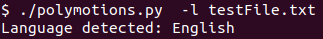
\includegraphics[width = 7cm, keepaspectratio]{Pictures/l.png}
    \caption{Exemplo de Funcionamento da deteção de idioma. }
    \label{fig:loption}
\end{center}
\end{figure}

\paragraph{Obtenção do sentimento de um dado texto:} Esta função do sistema devolve como \textit{output} o resultado do cálculo do sentimento de um dado texto. Este valor resulta da soma das polaridades de cada uma das palavras encontradas. É ainda devolvida a média do sentimento do texto (isto é possível uma vez que há medida que o texto é analisado, é feita uma contagem do número de palavras que este contem).
Esta funcionalidade é ativada  com a flag \verb|-t| ou com a \verb|-a| que ativa todas.
O código associado a esta função é o seguinte:

\begin{verbatim}
    def textSentiment(parsedText,lang):
        if allOp != None or textOp != None or fullOp != None:
            sumSentiment = 0
            numberWords = 0
            for word in parsedText.words:
                numberWords += 1
                sumSentiment += word.polarity
    
        if allOp != None or textOp != None:
            print("\nSentiment of text:")
            print("\tsum: " + str(sumSentiment))
            print("\tmean: " + str(sumSentiment/numberWords))

        return (sumSentiment,numberWords)
        
\end{verbatim}

Segue-se um exemplo do funcionamento da mesma.

\begin{figure}[H]
\begin{center}
    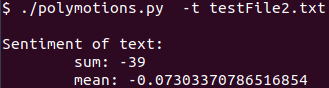
\includegraphics[width = 7cm, keepaspectratio]{Pictures/t.png}
    \caption{Exemplo de Funcionamento da obtenção do sentimento de um dado texto. }
    \label{fig:toption}
\end{center}
\end{figure}

\paragraph{Obtenção do sentimento das entidades de um texto:} Esta terceira opção tem como objetivo devolver o sentimento associado a cada ocorrência das entidades que constam num texto, fazendo-o por ordem de ocorrência destas no texto. Para tal, há dois elementos principais envolvidos, o Reconhecimento de Entidades e a Análise de Sentimento, uma vez que esta função não resulta se a língua do texto não for suportada por ambas as \textit{features} do Polyglot.
Segue-se um excerto do código relevante para a compreensão do funcionamento desta funcionalidade:
\begin{verbatim}
def entitiesAndFinalSentiment(parsedText,lang,sumSentiment,numberWords):

    print("\nSentiment associated to each entity by order of appearance in text:")
    
    for entity in parsedText.entities:
        entitySent = entity.positive_sentiment-entity.negative_sentiment

        print("\t" + str(" ".join(entity)) + ": " + str(entitySent))
\end{verbatim}

\begin{figure}[H]
\begin{center}
    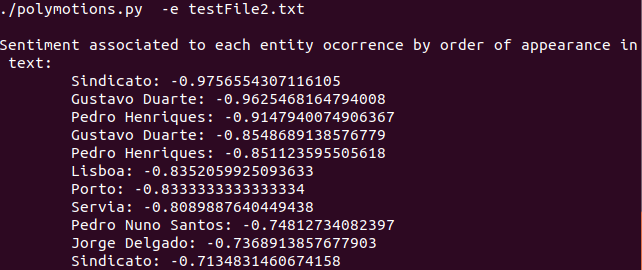
\includegraphics[width = 12cm, keepaspectratio]{Pictures/e.png}
    \caption{Exemplo de Funcionamento da obtenção do sentimento das entidades de um dado texto. }
    \label{fig:eoption}
\end{center}
\end{figure}

\paragraph{Obtenção do sentimento de uma entidade:} Esta funcionalidade devolve o valor do sentimento associado a uma dada entidade indicada pelo utilizador e que surja no texto \textit{input}. Concretamente, são devolvidos por cada ocorrência da mesma no texto o valor de sentimento e, por fim, o somatório e a média calculada desses valores.

\begin{verbatim}
def entitiesAndFinalSentiment(parsedText,lang,sumSentiment,numberWords):
    
    findsSent = 0
    findsOcur = 0
    findsOut = ""

    for entity in parsedText.entities:
        entitySent = entity.positive_sentiment-entity.negative_sentiment
        jEntity = " ".join(entity)
        if findOp in jEntity:
            findsOut += "\t" + jEntity + ": " + str(entitySent) + "\n"
            findsSent += entitySent
            findsOcur += 1

    print("\nOcurences and sentiment of \"" + findOp + "\" entity:")
        print(findsOut, end='')
    
    print("\nTotal of \"" + findOp + "\" entity:")
        print("\tsum: " + str(findsSent))
        print("\tmean: " + str(findsSent/findsOcur))
\end{verbatim}

\begin{figure}[H]
\begin{center}
    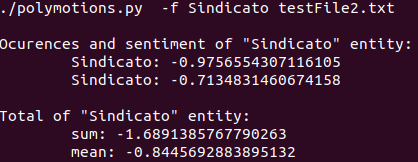
\includegraphics[width = 9cm, keepaspectratio]{Pictures/f.png}
    \caption{Exemplo de Funcionamento da obtenção do sentimento de uma entidade um dado texto. }
    \label{fig:foption}
\end{center}
\end{figure}

\paragraph{Comportamento \textit{default}:} O comportamento \textit{default} do sistema é ativado quando não se indica nenhuma flag. Como resultado devolve o somatório e a média do sentimento do texto, tendo em conta a noção de entidades. Isto é, faz a análise do sentimento do texto palavra a palavra (opção 1.Obtenção do sentimento de um dado texto) e soma com o valor do cálculo do sentimento de todas as entidades presentes no texto.
\begin{figure}[H]
\begin{center}
    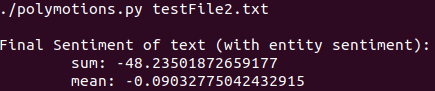
\includegraphics[width = 9cm, keepaspectratio]{Pictures/default.png}
    \caption{Exemplo de Funcionamento do comportamento \textit{default}. }
    \label{fig:doption}
\end{center}
\end{figure}

\paragraph{Opção com todas as funcionalidades:} Esta opção devolve 4 elementos, nomeadamente, os resultados de cada uma das quatro seguintes funcionalidades: deteção da linguagem de um dado texto, obtenção do sentimento de um dado texto, obtenção do sentimento das entidades de um texto e o resultado do comportamento default explicado previamente. A flag que deve ser utilizada para esta funcionalidade é a \verb|-a|. Esta é uma boa opção para quem pretende obter uma visão mais geral das \textit{features} do sistema, já que de uma só vez é possível visualizar quatro (em cinco) tipos de análises efetuadas ao texto. Convém ainda referir que esta opção pode ser utilizada com qualquer outra flag o que não impedirá o seu funcionamento. Uma sugestão seria o uso combinado \verb|-af xxxx| sendo \textit{xxxx} a entidade que se prentende analisar.

\begin{figure}[H]
\begin{center}
    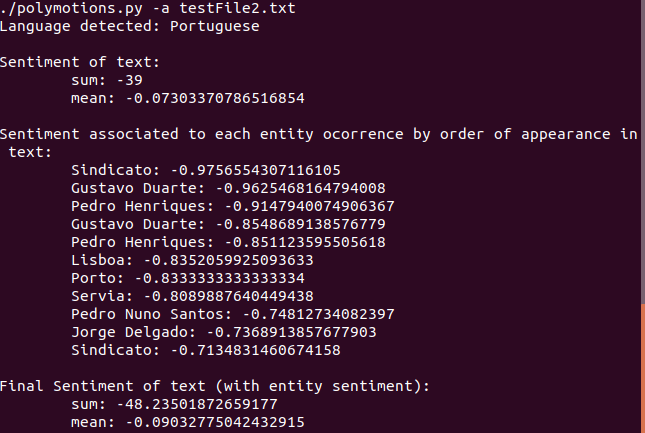
\includegraphics[width = 12cm, keepaspectratio]{Pictures/a.png}
    \caption{Exemplo de Funcionamento da opção com todas as funcionalidades. }
    \label{fig:aoption}
\end{center}
\end{figure}

Por fim, convém referir que os ficheiros que o sistema faz download são guardados numa pasta \textit{polyglot\_data} na \textit{home} do utilizador.

\section{Suporte para Português}

\quad Tal como mencionado anteriormente, o \textit{Polyglot} possui oito funcionalidades principais, cada uma delas disponível para um certo numero de línguas (desde 40 suportadas a nível do Reconhecimento de Entidades, até 196 na Deteção de Idioma).

No que toca à língua portuguesa, é possível descobrir quais as funcionalidades suportadas quer pelo website visitando as páginas relativas a cada uma das \textit{features}, quer através da biblioteca com a seguinte linha de código: \verb|downloader.supported_tasks(lang="pt")|. É também possível através do modo iterativo de download da linha de comandos (\verb|polyglot download|). 

É ainda possível listar as línguas suportadas para uma dada funcionalidade. Por exemplo, caso um utilizador quisesse saber quais os idiomas para os quais o Reconhecimento de Entidades pode ser usado, bastaria imprimir os resultados da seguinte forma:
\begin{verbatim}
    print(downloader.supported_languages_table(task="ner2"))    
\end{verbatim}
o que lhe devolveria a lista de \textit{output} pretendida.

Recorrendo a uma destas quatro alternativas facilmente se descobre as \textit{features} de que se pode tirar partido para utilizar em textos escritos em português. Deste modo, os itens suportados para a língua portuguesa são os seguintes:
\begin{itemize}
    \item Tokenização
    \item Deteção da língua de um texto
    \item Reconhecimento/extração de entidades mencionadas
    \item Identificação de categorias gramaticais (\textit{Part of Speech Tagging})
    \item Análise de Sentimento
    \item \textit{Embedding} de palavras
    \item Análise Morfológica
    \item Transliteração
\end{itemize}

Parte deste suporte é conseguido através do \textit{download} de ficheiros pelo Polyglot.

Podemos então concluir que para a língua portuguesa, todas as funcionalidades da framework são suportadas.


\section{Conclusões e Trabalho Futuro}
\qquad Após as implementações por nós feitas tendo como base o \textit{Polyglot} e as suas funcionalidades, surgiram-nos ideias que consideramos interessantes para exploração em futuros projetos. Concretamente, seria pertinente e possivelmente vantajoso usar a \textit{feature} de Análise de Sentimento como uma heurística para a deteção de \textit{fake news}, isto é, noticias falsas. 

Tal seria possível partindo do seguinte princípio: quando uma notícia possui um sentimento associado muito extremo (significativamente elevado ou reduzido) a probabilidade de ser \textit{biased} (tendenciosa) é maior uma vez que as notícias devem ser, à partida, neutras. Assim, os casos em que isto se verificasse, seriam sinalizados e seria devolvida uma percentagem da probabilidade de a noticia ser falsa.

Uma possível implementação para esta heurística seria semelhante à que é utilizada na deteção de línguas, por exemplo. Ou seja, seria vantajoso ter um ``dataset'' base com o sentimento de múltiplas notícias (falsas e verdadeiras), por forma a comparar com os sentimentos das notícias a analisar.

Por fim, consideramos que a realização deste trabalho nos permitiu adquirir mais conhecimentos acerca da ferramenta estudada, bem como conhecimentos na área de Processamento de Linguagens em geral. Quanto à \textit{framework} em si, fazemos uma avaliação positiva da mesma devido à facilidade de uso e à sua versatilidade. A nível do trabalho, acreditamos ter cumprido os objetivos e aprimorado as nossas competências na área tal como pretendido.


\printbibliography
\newpage


\begin{appendices}

\section{Menu de ajuda da interface via linha de comandos} \label{helpCMD}
\begin{verbatim}
usage: polyglot [-h] [--lang LANG] [--delimiter DELIMITER] [--workers WORKERS]
                [-l LOG] [--debug]
                {detect,morph,tokenize,download,count,cat,ner,pos,transliteration,sentiment}
                ...

optional arguments:
  -h, --help            show this help message and exit
  --lang LANG           Language to be processed
  --delimiter DELIMITER
                        Delimiter that seperates documents, records or even
                        sentences.
  --workers WORKERS     Number of parallel processes.
  -l LOG, --log LOG     log verbosity level
  --debug               drop a debugger if an exception is raised.

tools:
  multilingual tools for all languages

  {detect,morph,tokenize,download,count,cat,ner,pos,transliteration,sentiment}
    detect              Detect the language(s) used in text.
    tokenize            Tokenize text into sentences and words.
    download            Download polyglot resources and models.
    count               Count words frequency in a corpus.
    cat                 Print the contents of the input file to the screen.
    ner                 Named entity recognition chunking.
    pos                 Part of Speech tagger.
    transliteration     Rewriting the input in the target language script.
    sentiment           Classify text to positive and negative polarity.
\end{verbatim}

\end{appendices}

\end{document}
